%%
%% (
%%  )\ )                             (
%%  (()/(   (            (             )\  )   (
%%   /(_))  ))\   (       ))\  (   (   (()/(   ))\
%%   (_))  /((_)  )\  )  /((_) )\  )\   ((_))/((_)
%%   | _ \(_))(  _(_/( (_) )  ((_)((_)  _| |(_))
%%   |   /| || || ' \))/ -_)/ _|/ _ \/ _` |/ -_)
%%   |_|_\ \_,_||_||_| \___|\__|\___/\__,_|\___|
%%

\documentclass{article}
\usepackage[utf8x]{inputenc}
\usepackage{amsmath}
%\usepackage{slashbox}
\usepackage{amsfonts}
\usepackage{amssymb}
\usepackage{graphicx} % Paquete para incluir imágenes en el documento LaTeX
\usepackage{hyperref}
\hypersetup{
  colorlinks=true,
  linkcolor=blue,
  filecolor=magenta,
  urlcolor=cyan,
}
\urlstyle{same}
\usepackage{varwidth}

\newcommand\tab[1][1cm]{\hspace*{#1}}

\usepackage{multirow}

\usepackage[a4paper,rmargin=1.5cm,lmargin=1.5cm,top=1.5cm,bottom=1.5cm]{geometry}

\usepackage{pdfpages}

\usepackage{xcolor}
\usepackage{minted}
\setminted[css]{frame=lines, framesep=2mm, baselinestretch=1.2, rulecolor=\color{black!80},
                bgcolor=DarkGray,fontsize=\normalsize}
\usemintedstyle[css]{monokai}
\setminted[python]{frame=lines, framesep=2mm, baselinestretch=1.2, rulecolor=\color{black!80}, bgcolor=DarkGray}
\usemintedstyle[python]{monokai}
\setminted[java]{frame=lines, framesep=2mm, baselinestretch=1.2, rulecolor=\color{black!80}, bgcolor=DarkGray}
\usemintedstyle[java]{monokai}
\setminted[javascript]{frame=lines, framesep=2mm, baselinestretch=1.2, rulecolor=\color{black!80}, bgcolor=DarkGray}
\usemintedstyle[javascript]{monokai}
\setminted[php]{frame=lines, framesep=2mm, baselinestretch=1.2, rulecolor=\color{black!30}, bgcolor=LightGray}
\setminted[html]{frame=lines, framesep=2mm, baselinestretch=1.2, rulecolor=\color{black!30}, bgcolor=LightGray}
\setminted[bash]{baselinestretch=1.2,rulecolor=\color{black!30},bgcolor=LightGray}
\definecolor{LightGray}{gray}{0.90}
\definecolor{DarkGray}{gray}{0.1}
\definecolor{MidGray}{gray}{0.8}
\definecolor{codegreen}{rgb}{0,0.6,0}
\definecolor{codegray}{rgb}{0.5,0.5,0.5}
\definecolor{codepurple}{rgb}{0.58,0,0.82}
\definecolor{backcolour}{rgb}{0.95,0.95,0.92}
\setminted[json]{frame=lines, framesep=2mm, baselinestretch=1.2, rulecolor=\color{black!80}, bgcolor=DarkGray}
\usemintedstyle[json]{monokai}
\setminted[apacheconf]{frame=lines, framesep=2mm, baselinestretch=1.2, rulecolor=\color{black!30}, bgcolor=LightGray}
\setminted[html+twig]{frame=lines, framesep=2mm, baselinestretch=1.2, rulecolor=\color{black!30}, bgcolor=LightGray}
\setminted[html+php]{frame=lines, framesep=2mm, baselinestretch=1.2, rulecolor=\color{black!30}, bgcolor=LightGray}

\setlength{\parindent}{0px}  % Setea la indentacion de la primera linea de cada parrafo a cero pixeles.


\title{Programación en Python 2}
\author{@RuneCode}

\begin{document}
%% Portada
\includepdf{./portada/portada.pdf}

%% Clase previa #1
\section{Instalación de anaconda}%

Para descargar anaconda puedes visitar el siguiente
\href{https://www.anaconda.com/}{enlace}.

\begin{figure}[h!]
  \centering
  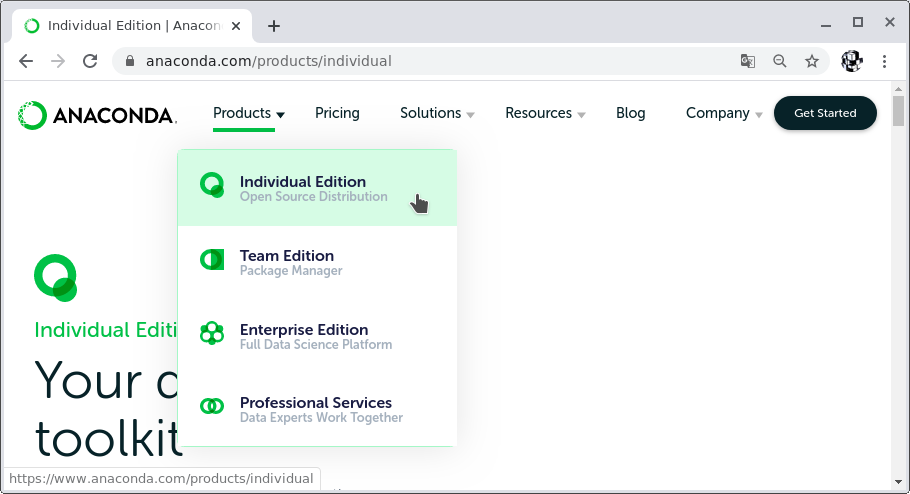
\includegraphics[scale=0.75]{./Pictures/001_install_anaconda.png}
\end{figure}

\begin{figure}[h!]
  \centering
  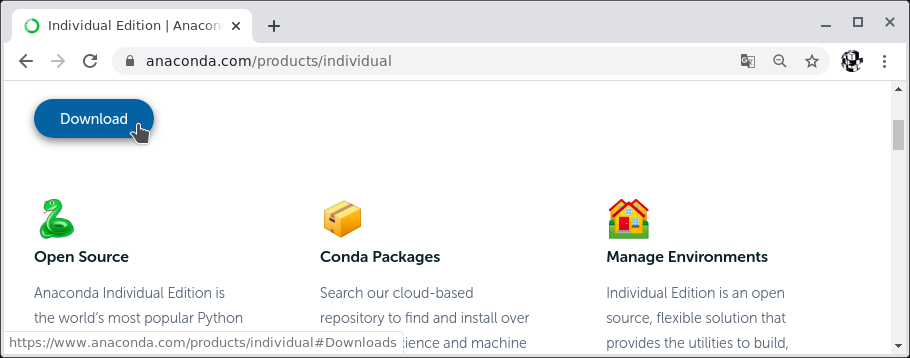
\includegraphics[scale=0.75]{./Pictures/001_download_anaconda.png}
\end{figure}

\newpage

\begin{figure}[h!]
  \centering
  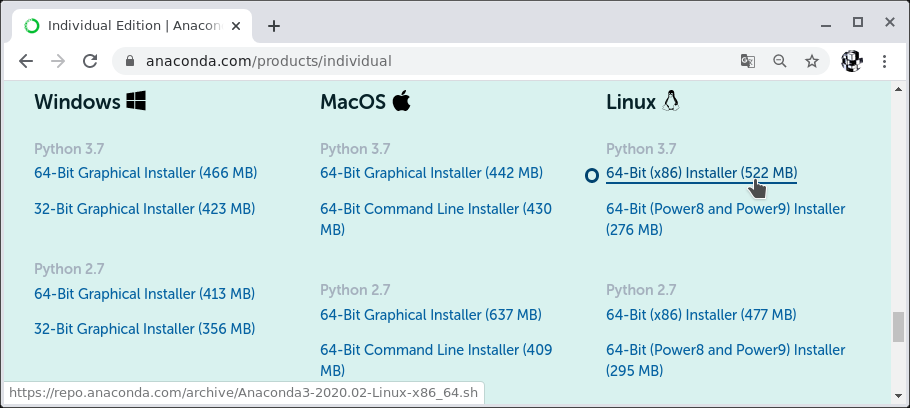
\includegraphics[scale=0.75]{./Pictures/002_download_anaconda.png}
\end{figure}

Al descargar obtendremos un script bash llamado
\textbf{Anaconda3-2020.02-Linux-x86\_64.sh}. Para poder ejecutarlo agregamos el
permiso de ejecución usando \textbf{chmod}\\

\begin{minted}{bash}
  chmod 755 Anaconda3-2020.02-Linux-x86_64.sh
  ./Anaconda3-2020.02-Linux-x86_64.sh
\end{minted}


\begin{figure}[h!]
  \centering
  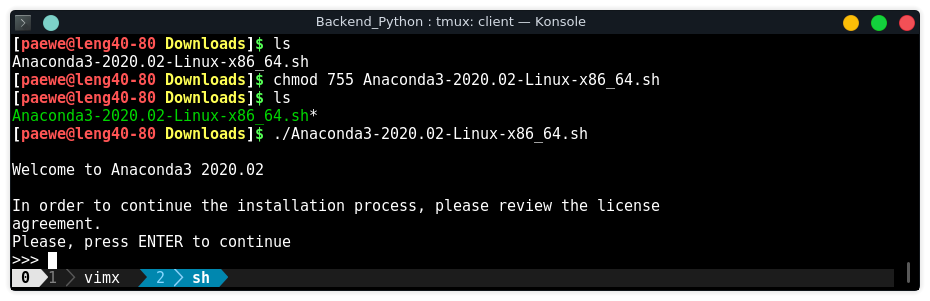
\includegraphics[scale=0.75]{./Pictures/003_install_anaconda.png}
\end{figure}

Para recorrer el acuerdo de licencia debes presionar la tecla \textbf{Espacio}
varias veces.

\begin{figure}[h!]
  \centering
  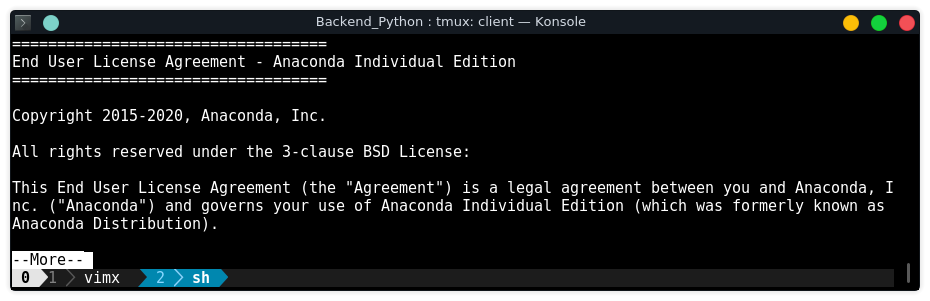
\includegraphics[scale=0.75]{./Pictures/004_licencia_more.png}
\end{figure}

\newpage

Para aceptar los terminos de la licencia escribimos \textbf{yes}.

\begin{figure}[h!]
  \centering
  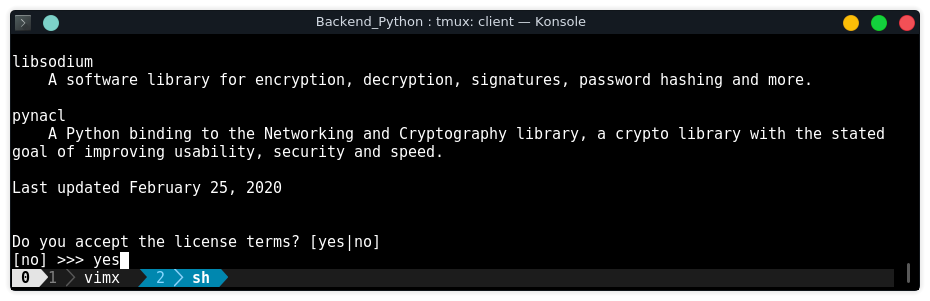
\includegraphics[scale=0.75]{./Pictures/005_aceptar_licencia.png}
\end{figure}

Luego escogemos un locación donde guardaremos anaconda o si queremos
simplemente presionamos \textbf{Enter} para usar la locación por defecto.

\begin{figure}[h!]
  \centering
  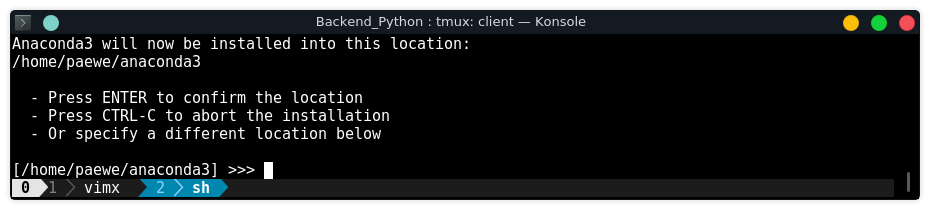
\includegraphics[scale=0.75]{./Pictures/006_install_location.png}
\end{figure}

Escogemos la opción \textbf{yes} para iniciar anaconda cada vez que se inicie
bash.

\begin{figure}[h!]
  \centering
  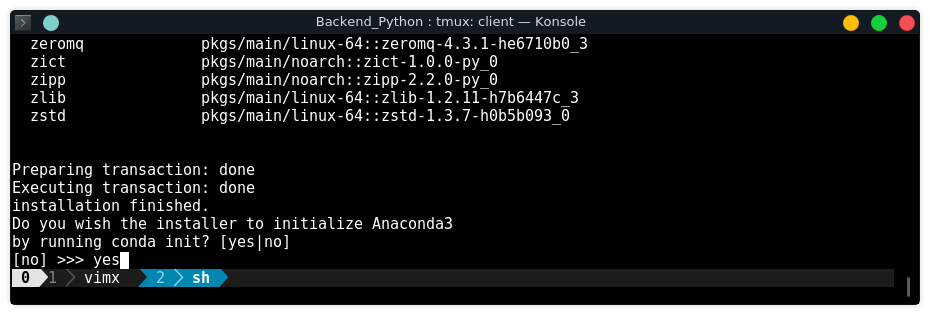
\includegraphics[scale=0.75]{./Pictures/007_iniciar_bash.png}
\end{figure}

Finalmente con esto ya se ha completado la instalación. Pero podemos configurar conda para que aunque se inicie no nos muestre el mensaje \textbf{base} en la parte izquierda del prompt. Para eso usamos:

\begin{minted}{bash}
  conda config --set changeps1 False
\end{minted}

Esto nos crea un archivo llamado \textbf{.condarc} que guarda las
configuraciones usados por conda.

\newpage

\begin{figure}[h!]
  \centering
  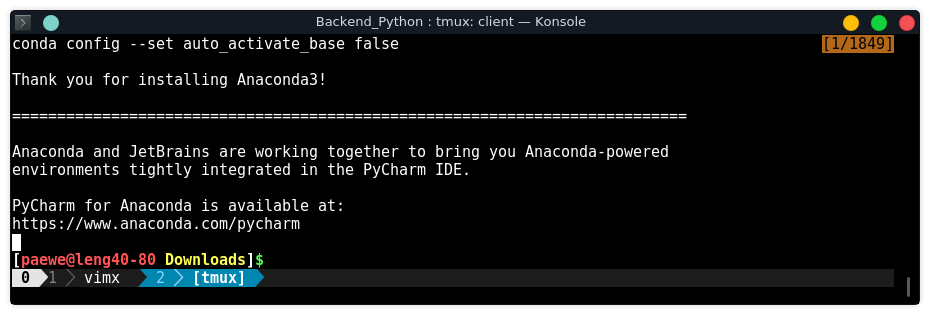
\includegraphics[scale=0.75]{./Pictures/008_instalacion_finalizada.png}
\end{figure}

\begin{figure}[h!]
  \centering
  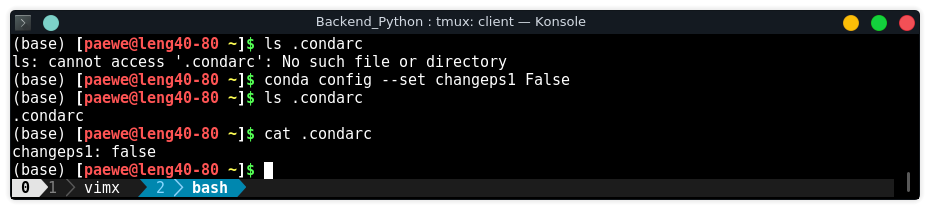
\includegraphics[scale=0.75]{./Pictures/009_changeps1_false.png}
\end{figure}

\newpage

%% Clase previa #2
\section{Instalación de un nuevo entorno con python2}%

Ya que hemos descargado \textbf{Anaconda} con la versión de Python 3.7, si
queremos usar otra versión de Python podemos crear un nuevo entorno con la
versión que usaremos. Para mayor información puedes revisar la documentación de
\textbf{Conda} en el siguiente
\href{https://docs.conda.io/projects/conda/en/latest/user-guide/tasks/manage-environments.html#creating-an-environment-with-commands}{enlace}.\\

Escribimos el siguiente comando:

\begin{minted}{bash}
  conda create -n python2 python=2.7
\end{minted}

\begin{figure}[h!]
  \centering
  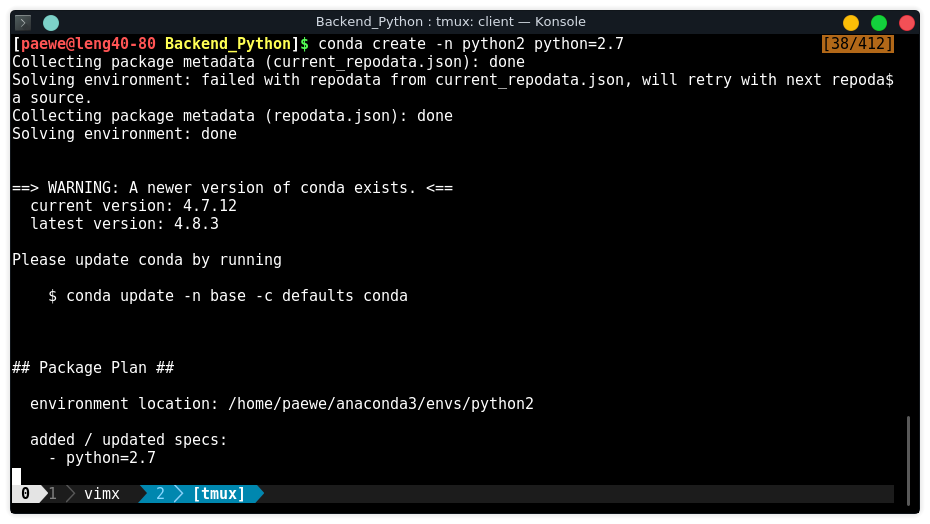
\includegraphics[scale=0.75]{./Pictures/001_crear_env_python2.png}
\end{figure}

\begin{figure}[h!]
  \centering
  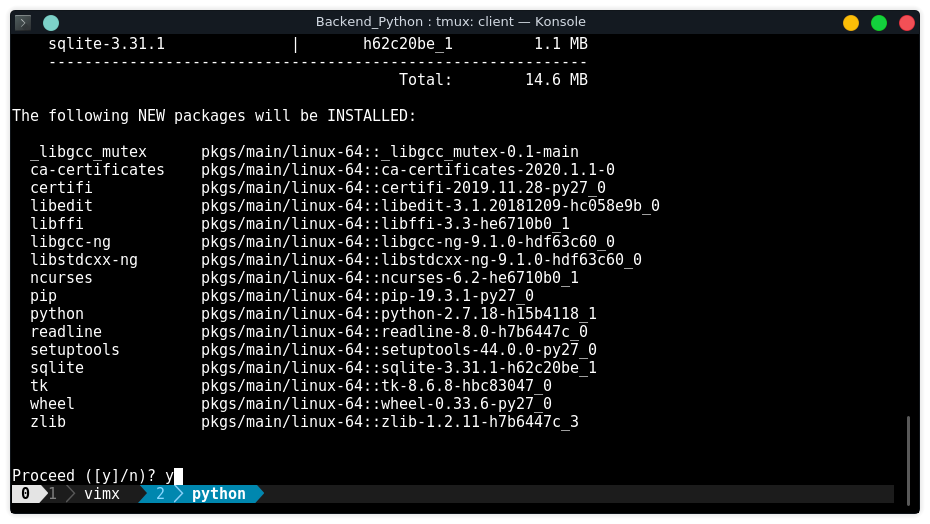
\includegraphics[scale=0.75]{./Pictures/002_crear_env_python2.png}
\end{figure}

\newpage

\begin{figure}[h!]
  \centering
  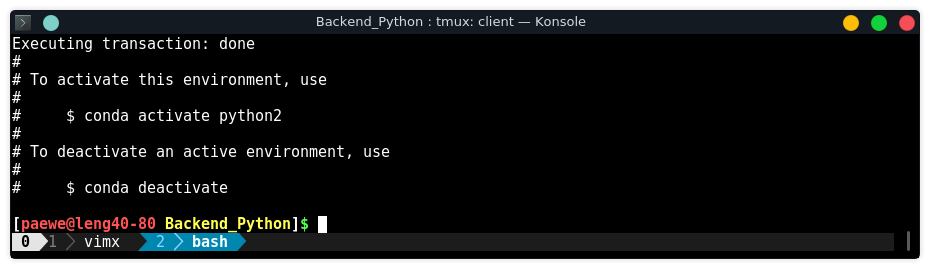
\includegraphics[scale=0.75]{./Pictures/003_crear_env_python2.png}
\end{figure}

Para activar el entorno que creamos usamos el siguiente comando.

\begin{minted}{bash}
  conda activate python2
\end{minted}

De igual manera, si queremos desactivar este entorno y usar el predeterminado
con Python 3.7, entonces usamos:

\begin{minted}{bash}
  conda deactivate
\end{minted}


\begin{figure}[h!]
  \centering
  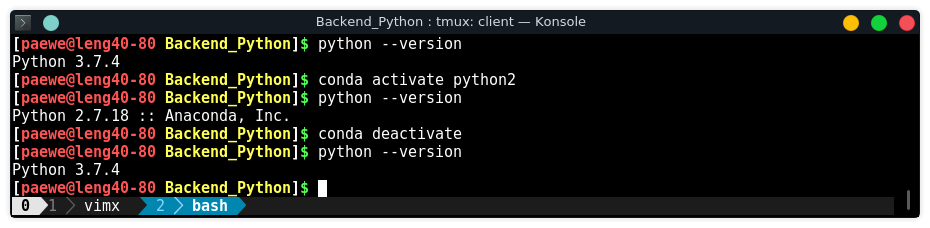
\includegraphics[scale=0.75]{./Pictures/004_activar_python2_desactivar.png}
\end{figure}

Si queremos ver los entornos que tenemos creados con Anaconda usamos el
siguiente comando:

\begin{minted}{bash}
  conda env list
\end{minted}


\begin{figure}[h!]
  \centering
  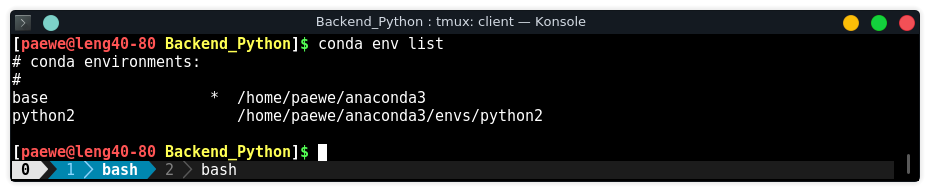
\includegraphics[scale=0.75]{./Pictures/005_ver_entornos_conda.png}
\end{figure}

\newpage

%% Clase 1
\section{¿Por qué programar con Python?}%
\subsection{¿Por qué?}%
Python es un lenguaje bastante bueno para aprender a programar ya que tiene una
comunidad muy grande que te ayudará a superar tus dudas, tiene una sintaxis
para escribir bastante sencilla.

\subsection{¿Qué es programar?}%
Programar es darle instrucciones al computador, para hacer algo que tu quieres,
desde tu sitio web a llevar humanos a marte.\\

Para lograr construir lo que quieres debes unir piezas básicas del lenguaje y
dependiendo de como las unas vas a construir eso que imaginas.\\

Para crear tu primer hola mundo debes encender el intérprete del Python, este
hola mundo es muy sencillo, ejecuta la función print así:

\begin{figure}[h!]
  \centering
  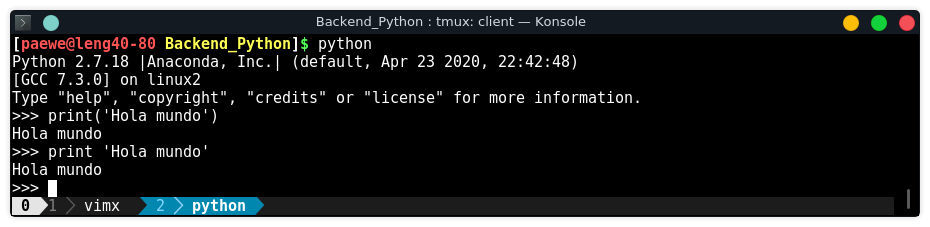
\includegraphics[scale=0.75]{./Pictures/005_hola_mundo_python2.png}
\end{figure}














































%% Clase 11
\section{Buena prácticas de lenguaje}%

\textbf{genero.py}
\begin{minted}{python}
  # -*- coding: utf-8 -*-

  genero = raw_input("Ingresa tu genero: ")
  edad = int(raw_input("Ingresa tu edad: "))

  if genero == 'masculino':
      if edad > 18:
          print 'Hola, señor.'
      else:
          print 'Hola niño.'
  else:
      if edad > 18:
          print 'Hola, señora.'
      else:
          print 'Hola niña.'
\end{minted}


%% Clase 12
\section{Comparación de strings y unicode}%

Los string son inmutables.
\begin{figure}[h!]
  \centering
  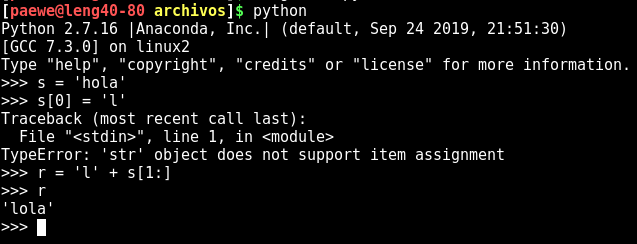
\includegraphics[scale=0.75]{./Pictures/001_string_inmutable.png}
\end{figure}

Se comparan los strings

\begin{figure}[h!]
  \centering
  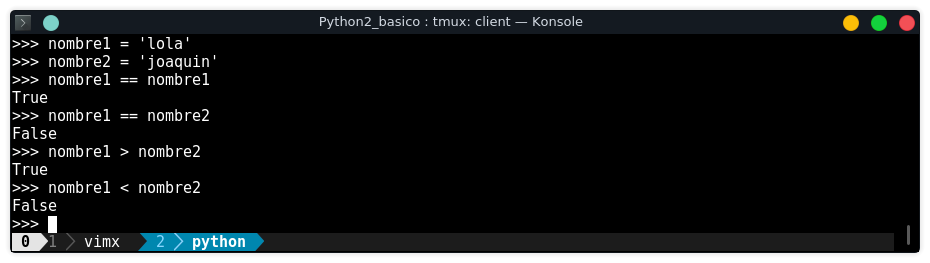
\includegraphics[scale=0.75]{./Pictures/002_comparar_strings.png}
\end{figure}

Escribir strings unicode en python 2.

\begin{figure}[h!]
  \centering
  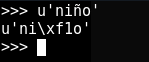
\includegraphics[scale=0.75]{./Pictures/003_unicode_python2.png}
\end{figure}



%% Clase 13
\section{Factorial de un número con recursión}%

\textbf{factorial.py}
\begin{minted}{python}
  # -*- coding: utf-8 -*-

  def factorial(number):
      if number == 0:
          return 1

      return number * factorial(number - 1)


  if __name__ == '__main__':
      number = int(raw_input('Ingrese el número: '))
      result = factorial(number)

      print(result)
\end{minted}


%% Clase 14
\section{Manejo de strings en Python}%
Un string es una secuencia de caracteres, donde cada caracter tiene un indice
que inicia en cero por ejemplo:


\begin{figure}[h!]
  \centering
  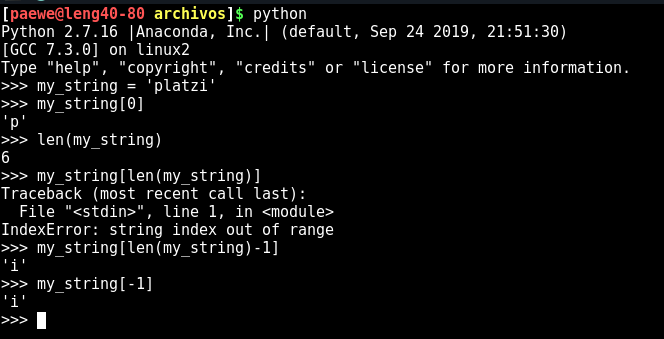
\includegraphics[scale=0.75]{./Pictures/004_index_string_len.png}
\end{figure}

\begin{itemize}
  \item upper
  \item iupper
  \item lower
  \item islower
  \item find
  \item isdigit
  \item endswith
  \item startswith
  \item split
  \item join
\end{itemize}

\begin{figure}[h!]
  \centering
  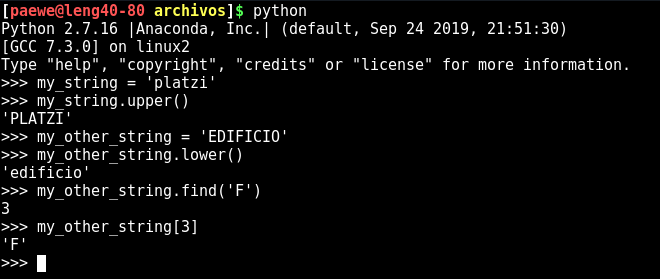
\includegraphics[scale=0.75]{./Pictures/005_methods_string.png}
\end{figure}






























\end{document}

